\documentclass[11pt, a4paper]{article}

% Encoding & fonts
\usepackage[T1]{fontenc}

% Layout & graphics
\usepackage{geometry}
\geometry{tmargin=0.8in,bmargin=0.8in,lmargin=0.8in,rmargin=0.8in,headsep=0.0in,headheight=0.5in,foot=30.0pt}
\usepackage{graphicx}
\usepackage{subcaption}

% Tables, colors
\usepackage{booktabs}
\usepackage[table,xcdraw]{xcolor}
\usepackage{longtable}
\usepackage{float}
\usepackage{array}

% Paragraph spacing
\usepackage{parskip}

% Hyperlinks
\usepackage[hidelinks]{hyperref}
\hypersetup{
    colorlinks=true,
    linkcolor=blue,
    filecolor=blue,
    urlcolor=blue,
    citecolor=blue
}

% Bibliography
\usepackage[style=apa, backend=biber]{biblatex}
\DeclareLanguageMapping{english}{english-apa}
\addbibresource{references.bib}

\title{Vision-Language-Action Models for Chemical Manipulation:\\
A Practical Study with SmolVLA on the SO-101 Robotic Arm}
\author{
    Ferdinand Paar \\[4pt]
    \small Student Nr.: s1128559 \quad Course: BKI209 (6 EC) \\
    \small Primary Supervisor: Andrei Voinea \quad
    Project Oversight: Dr.\ Mathijs Mabesoone \\
    \small Radboud University, Faculty of Social Sciences, AI Department
}
\date{June 2026}

\begin{document}

\maketitle

\begin{abstract}
Lab robots like the OT-2 use hard-coded coordinates and break if anything moves. Vision-Language-Action (VLA) models could help by letting the robot learn from examples instead of hand-coded rules. I tested a small VLA model, SmolVLA-450M, on an SO-101 robot doing a tube-in-hole task. For the final run, I trained on 50 episodes selected after more than 300 total recorded episodes during setup and testing, and fine-tuned the model on an A100 GPU. I tested how it handled position changes, lighting changes, and camera angle changes. The model got 9 out of 10 trials right when conditions matched training, but only 5 out of 10 when the tube was in a new position. Lighting did not matter much. Moving the camera even slightly broke the policy. The main problems were position-specific visual behaviour and a gripper that is not well suited for tubes. Project files are available in a private GitHub repository: \href{https://github.com/FerdinandPaar/so101-smolvla-pipe-in-hole}{so101-smolvla-pipe-in-hole}. The dataset and trained model are available on Hugging Face Hub: \href{https://huggingface.co/datasets/mundgelenk/so101_50_pipe_in_hole}{dataset} and \href{https://huggingface.co/mundgelenk/smolvla_so101_pipe_in_hole}{model}.
\end{abstract}

\tableofcontents
\newpage

%% ----------------------------------------------------------------
\section{Introduction}
\label{sec:intro}
%% ----------------------------------------------------------------

Laboratory automation has become central to modern chemistry, where liquid-handling robots such as the Opentrons OT-2 carry out repetitive pipetting and sample-transfer steps with high throughput and reproducibility \parencite{bolt2025platehandler}. These platforms are coordinate controlled: every motion is specified as a fixed sequence of coordinates on a calibrated deck. This works well as long as the physical layout never changes, but it makes the system brittle. If a tube rack is nudged, a vial is slightly tilted, or a consumable is placed a few millimetres off its expected location, the robot cannot notice or adapt. It executes the same coordinates regardless, and the step fails until a human re-calibrates the deck. In a busy, shared laboratory where set-ups are reconfigured between experiments, this rigidity is a recurring source of failure and manual intervention.

An alternative is to let the robot perceive its workspace and react to it, rather than follow fixed coordinates. Vision-Language-Action (VLA) models are a recent class of neural network that make this possible: instead of being programmed with coordinates, the robot is given a camera image and a short task description and predicts the motor commands directly \parencite{shukor2025smolvla}. Because VLAs are trained from human demonstrations rather than hand-written rules, an approach known as imitation learning \parencite{hussein2017imitation}, the hope is that they generalise across the small layout variations that break a coordinate-based system, without any reprogramming. VLAs originated in general-purpose manipulation research, such as picking, sorting, and tool use, but their tolerance for visual variation makes them an attractive candidate for the semi-structured environment of a chemistry lab.

Whether that promise holds for a realistic lab task, on affordable hardware, is far from obvious. Compact VLAs are trained on a limited number of demonstrations and may simply memorise the scenes they were shown rather than learn to locate objects. If so, the very brittleness we hoped to remove would reappear in a different form, as sensitivity to object position, lighting, or camera placement. Establishing which of these perturbations a small VLA can absorb, and which break it, is therefore a prerequisite for judging whether VLAs are a viable path toward flexible lab automation.

This project tests that question in a practical setup. I fine-tuned SmolVLA-450M \parencite{shukor2025smolvla}, a compact open-source VLA designed to run on consumer hardware, on an SO-101 home-lab arm, a low-cost 6-axis robotic arm for imitation-learning research. The task was pipe-in-hole: picking up a test tube and inserting it into a rack slot as a simplified stand-in for the tube-transfer steps performed on OT-2-style equipment. I then measured how its performance changed under the kinds of perturbation a real lab introduces.

Research question: Can a compact VLA (SmolVLA-450M), fine-tuned on 50 demonstrations, keep reliable pipe-in-hole performance when object position, lighting, and camera viewpoint change in ways typical of a shared chemistry lab?

I address this through four experiments: a baseline under training-matched conditions (Section~\ref{sec:baseline}), and controlled perturbations of object starting position (Section~\ref{sec:pos}), lighting (Section~\ref{sec:lighting}), and camera viewpoint (Section~\ref{sec:camerapos}). Together these isolate which sources of variation a small VLA tolerates and which it does not.

The remainder of the report is organised as follows. Section~\ref{sec:background} introduces VLAs, the role of task-naming, and the SmolVLA model. Section~\ref{sec:setup} describes the hardware, the task, and the data-collection and training procedure. Section~\ref{sec:results} reports the four experiments. Section~\ref{sec:discussion} analyses the observed failure modes, and Section~\ref{sec:limitations} discusses limitations and future work. Section~\ref{sec:conclusion} concludes.

%% ----------------------------------------------------------------
\section{Background}
\label{sec:background}
%% ----------------------------------------------------------------

\subsection{Vision-Language-Action Models}

A VLA is a unified neural network that simultaneously processes three streams of information to produce robot actions \parencite{hussein2017imitation, shukor2025smolvla}:

\begin{itemize}
    \item \textbf{Vision:} Real-time RGB image frames from one or more robot-mounted cameras.
    \item \textbf{Language:} A text string describing the task to be executed.
    \item \textbf{Action:} A predicted sequence of joint positions or velocities, called an action chunk, that the robot should execute.
\end{itemize}

Unlike classical pipelines that use separate modules for detection, planning, and control, a VLA does all three at once \parencite{rothman2024transformers}. This reduces error buildup and makes the system more robust to camera noise and small object changes, which matters in labs where the deck layout changes.

Image understanding in these systems is not just a text-only LLM reading pixels. It is a separate research area with a different architecture: the model needs a vision encoder and projection layers to turn images into representations that can be combined with language and then mapped to robot actions \parencite{shukor2025smolvla, rothman2024transformers}.

\subsection{Task-Naming as Behavioural Switching}

A common misconception is that current compact VLA models understand natural language in the way a large language model does. In practice, models like SmolVLA use task-naming as a categorical switch rather than performing semantic parsing.

During training the model learns to map a specific text string to a specific motor behaviour. The text is like a lookup key: the string \texttt{"pick\_lego"} activates weights for block-grasping, while \texttt{"wipe\_table"} activates weights for sweeping.

The limitation is that a different wording from training can fail because it no longer matches the learned task key. So in practice, you need to use the exact same task name every time.

One solution is to place a language model upstream of the VLA. The LLM rewrites free-form requests into the exact task-name strings used during training. This two-stage pipeline could work well for OT-2 chemistry workflows where operators might phrase things differently across sessions.

\subsection{SmolVLA-450M}
\label{sec:smolvla}

SmolVLA-450M \parencite{shukor2025smolvla} is an open-source, lightweight VLA model developed by Hugging Face for the LeRobot ecosystem. It is designed to run on consumer hardware like a MacBook or cheap GPU, making it practical for a student project.

The key advantage is that it predicts chunks of future actions, about 50 timesteps, rather than single actions. This makes robot movements smoother because the policy does not need to decide every motor command independently. For this project, the main constraint was inference. Training could run on the A100 cluster, but deployment had to run beside the robot on my MacBook M1 Pro. The cluster would only solve this bottleneck if I had a low-latency inference tunnel working: the MacBook would send RGB images and joint positions to the cluster, and the cluster would send back the next motor command in time. I did not get that tunnel working, so the model still had to be small enough for local inference.

%% ----------------------------------------------------------------
\section{Experimental Setup}
\label{sec:setup}
%% ----------------------------------------------------------------

\subsection{Hardware}

\subsubsection*{SO-101 Robotic Arm System}

The SO-101 is an open-source 6-axis robotic arm designed for imitation-learning research (Figure~\ref{fig:so101}). It has these parts:

\begin{itemize}
    \item \textbf{Leader arm:} A passive, low-friction arm moved by hand to record demonstrations during data collection.
    \item \textbf{Follower arm:} The active arm that mirrors the leader during collection and operates autonomously during inference.
    \item \textbf{Feetech STS3215 servos:} Magnetic absolute encoders provide high-precision joint-position feedback at each of the six degrees of freedom.
    \item \textbf{Dual-camera setup:} One overhead camera (front workspace view) and one wrist-mounted camera, providing the two visual streams required by SmolVLA.
\end{itemize}

\begin{figure}[H]
    \centering
    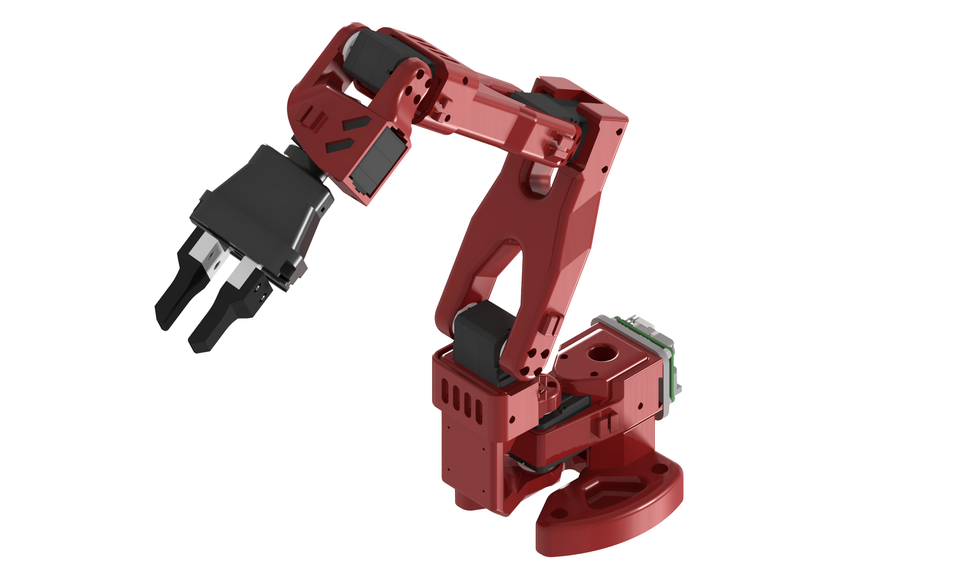
\includegraphics[width=0.45\textwidth]{images/SO-101.png}
    \caption{The SO-101 follower arm used in this project.}
    \label{fig:so101}
\end{figure}

\subsubsection*{Compute}

Inference was run on a MacBook M1 Pro (16\,GB unified memory). Fine-tuning was launched on a compute node with four NVIDIA A100 40\,GB GPUs; the final training run used one of those GPUs.

\subsubsection*{Home-Lab Environment}

I set up the SO-101 with dual cameras and a test-tube rack as a home-lab testbed (Figure~\ref{fig:homelab}). It mimics an OT-2 deck: small working area, different-sized objects, and a target slot that the robot has to find visually.

\begin{figure}[H]
    \centering
    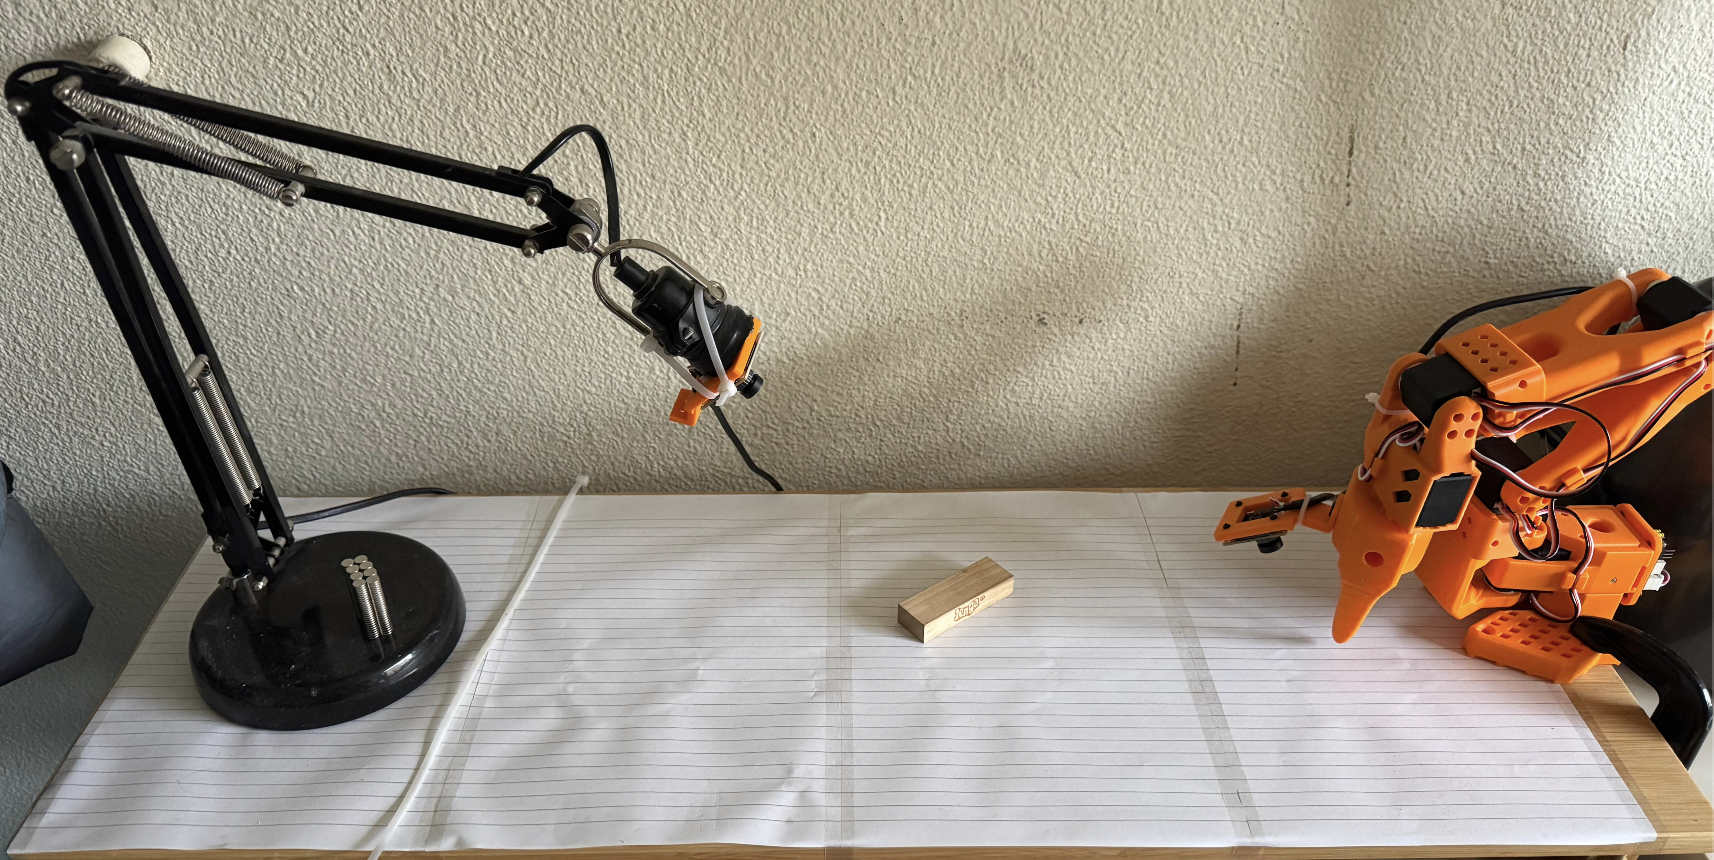
\includegraphics[width=0.7\textwidth]{images/Home Lab setup.png}
    \caption{Home-lab testbed. The overhead camera provides a front workspace view; the wrist camera travels with the end-effector.}
    \label{fig:homelab}
\end{figure}

\subsection{Task Design and Data Collection}

\subsubsection*{Task: Pipe-in-Hole}

The target task was pipe-in-hole: pick up a test tube from a small stand and insert it into a larger hole in a rack (Figure~\ref{fig:setup_topview}). This task has the key challenges of lab manipulation: grasping a small cylinder, placing it accurately in a slot, and finding it under different lighting. The task label was \texttt{"Pipe in hole"}.

\begin{figure}[H]
    \centering
    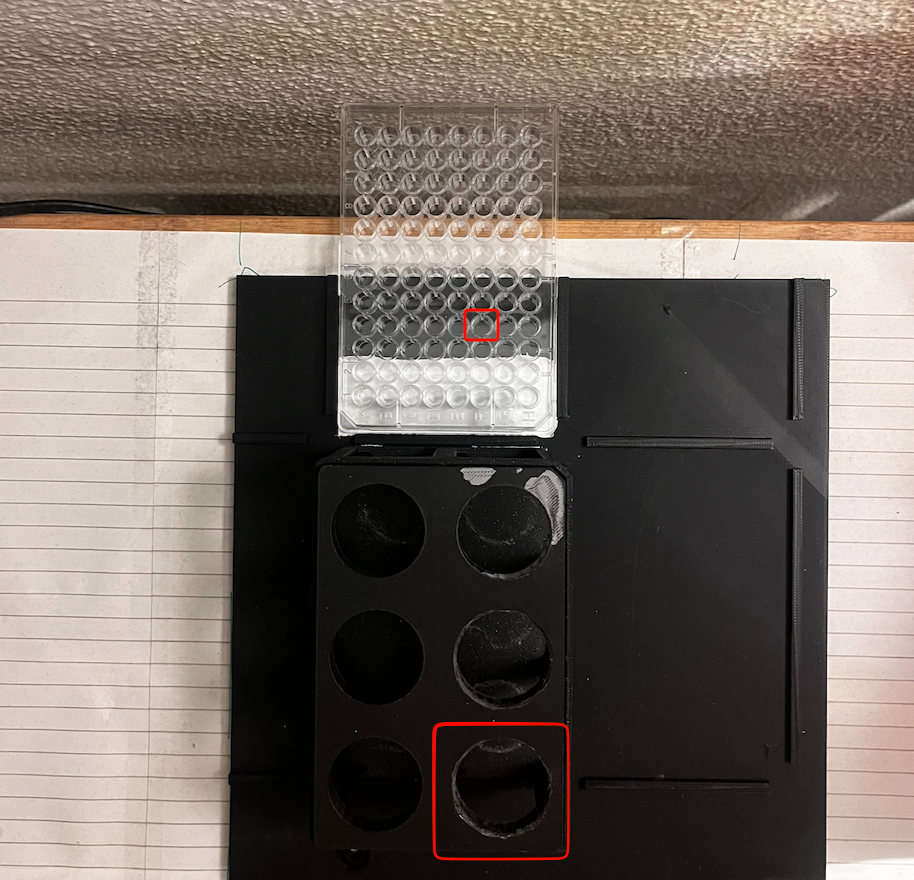
\includegraphics[width=0.42\textwidth]{images/gripper_angular.png}
    \caption{Top view of the experimental setup. The upper red square marks the tube starting position, and the larger lower red square marks the goal position for the tube.}
    \label{fig:setup_topview}
\end{figure}

\subsubsection*{Data Collection}

I recorded more than 300 episodes in total while building and debugging the setup. A lot of those recordings were learning runs: I adjusted camera placement, lighting, reset timing, gripper approach, and the episode workflow. For the final training run, I trained on 50 episodes recorded with the LeRobot \texttt{lerobot-record} script. Each time, I controlled the follower arm with the leader arm while watching the camera. I only watched the camera, not the physical robot, so the model would have the same information at inference time.

Figures~\ref{fig:data1} and \ref{fig:data2} show how episodes varied naturally. The tube was at different angles, the approach was from different directions, tube rotation was different each time. This wasn't planned but it's realistic. But as Section~\ref{sec:pos} shows, I still didn't cover all the positions.

\begin{figure}[H]
    \centering
    \begin{subfigure}[b]{0.46\textwidth}
        \centering
        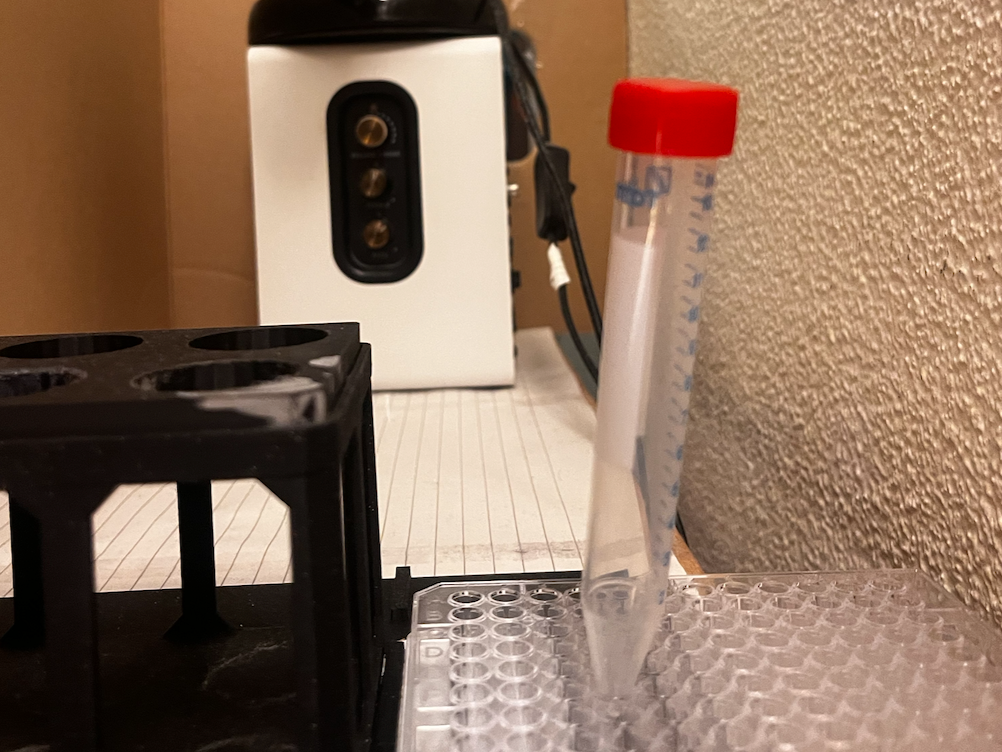
\includegraphics[width=\textwidth]{images/training_data_1.png}
        \caption{Episode: one tube orientation.}
        \label{fig:data1}
    \end{subfigure}
    \hfill
    \begin{subfigure}[b]{0.46\textwidth}
        \centering
        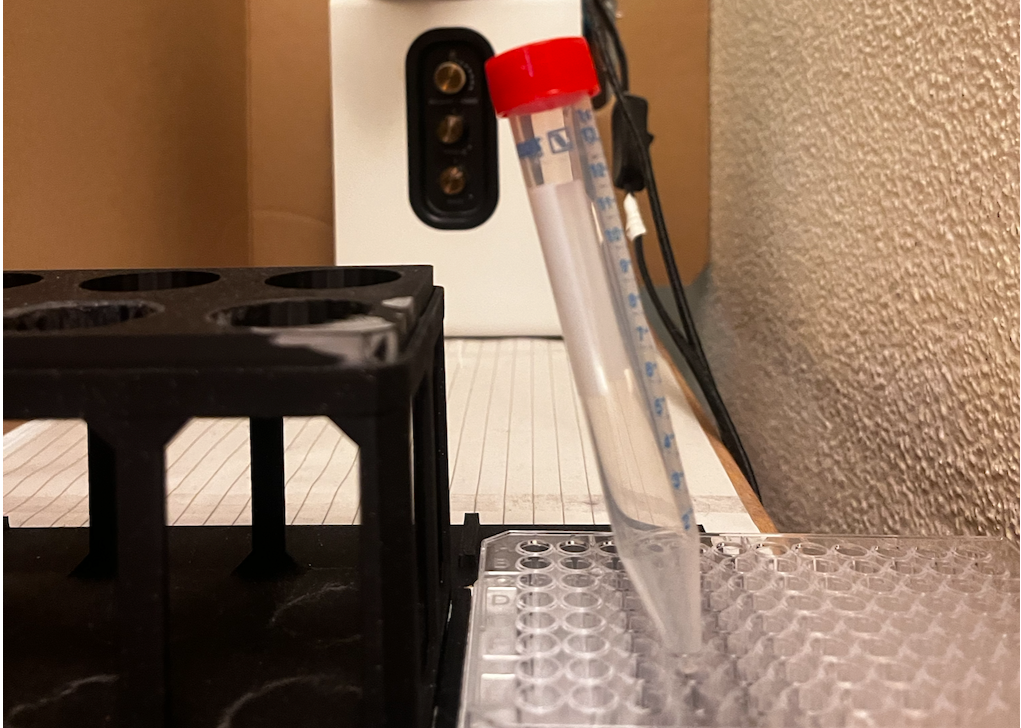
\includegraphics[width=\textwidth]{images/training_data_2.png}
        \caption{Episode: a different tube orientation.}
        \label{fig:data2}
    \end{subfigure}
    \caption{Variance across training demonstrations. Tube position and gripper approach angle differed between episodes, introducing natural noise into the dataset.}
    \label{fig:training_data}
\end{figure}

\subsection{Training}

Fine-tuning was performed with the LeRobot \texttt{lerobot-train} script. Key hyperparameters:

\begin{itemize}
    \item \textbf{Base model:} \texttt{lerobot/smolvla\_base}
    \item \textbf{Batch size:} 16
    \item \textbf{Training steps:} 30{,}000
    \item \textbf{Mixed precision:} AMP (bfloat16)
    \item \textbf{Checkpoint frequency:} Every 2{,}500 steps
\end{itemize}

I uploaded the dataset and trained model to Hugging Face Hub: \href{https://huggingface.co/datasets/mundgelenk/so101_50_pipe_in_hole}{dataset repository} and \href{https://huggingface.co/mundgelenk/smolvla_so101_pipe_in_hole}{model repository}.

I logged training to Weights \& Biases; the individual metric curves are reproduced in Appendix~\ref{app:training}. The main signals indicated a clean, stable run:

\begin{itemize}
    \item \textbf{Training loss} (Figure~\ref{fig:training-overview}) decreased from roughly 0.08 to about 0.01 and then flattened.
    \item \textbf{Gradient norm} (Figure~\ref{fig:training-overview}) stayed bounded, which suggests numerically stable optimisation.
    \item \textbf{Learning rate} (Figure~\ref{fig:training-overview}) followed the expected warm-up-then-decay schedule.
    \item \textbf{Resource use} (Figures~\ref{fig:system-overview} to~\ref{fig:node-io}) stayed stable during the run.
\end{itemize}

%% ----------------------------------------------------------------
\section{Results}
\label{sec:results}
%% ----------------------------------------------------------------

I tested the model on the MacBook M1 Pro. Each test had 10 tries. Success meant the tube got fully inserted into the hole without me having to help.

\subsection{Baseline: Training-Matched Conditions}
\label{sec:baseline}

When I used the same lighting, camera position, and tube placement as in training, the model succeeded 9 out of 10 times.\footnote{Example: \url{https://youtu.be/NdbsRoq-Wh8}.} The one failure happened because the gripper slipped slightly during approach, which is a known problem with the angular gripper design (Section~\ref{sec:gripper}).

This baseline result is encouraging for a small student setup. It suggests that VLA-based tube transfer can work on cheap hardware when the inference scene matches the training scene closely.

\subsection{Sensitivity to Object Starting Position}
\label{sec:pos}

I tested what happens when the tube is in a position that was never in the training data. Several slots in the test rack (shown in yellow in Figure~\ref{fig:startpos}) didn't appear in any of the 50 training episodes.

\begin{figure}[H]
    \centering
    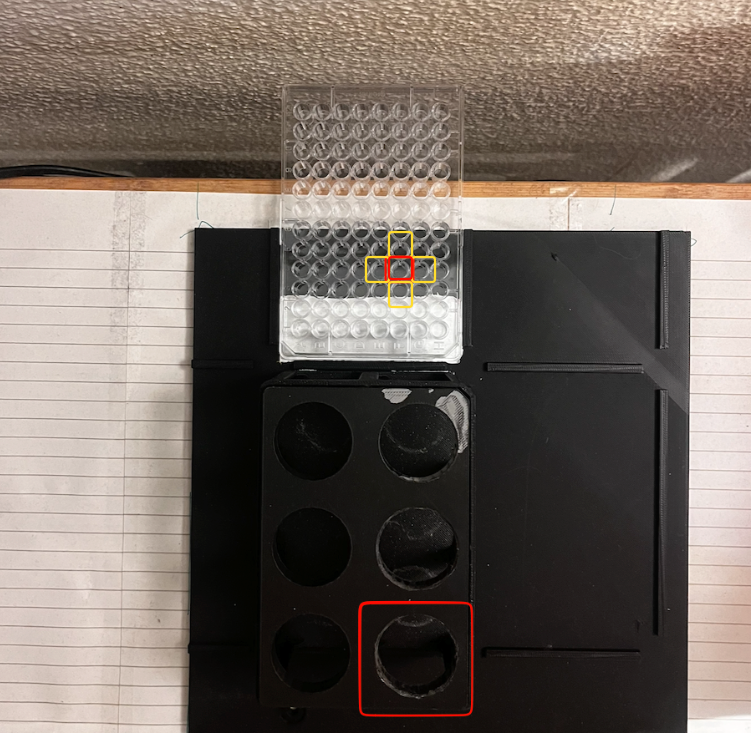
\includegraphics[width=0.55\textwidth]{images/starting_position.png}
    \caption{Yellow fields indicate tube starting positions absent from the training data. Placing the tube in these slots reduced success from 9/10 to 5/10.}
    \label{fig:startpos}
\end{figure}

Accuracy dropped to 5 out of 10. The arm often reached toward the area where the tube usually appeared during training, even when I placed it somewhere else. This does not mean the model learned nothing about the tube; it more likely learned a mix of tube recognition and a strong bias toward familiar image locations.

So the model struggles when the tube is in a new position. The problem is that my final 50 training episodes did not cover enough different regions of the rack, so the action policy stayed tied too closely to the positions it had seen. Section~\ref{sec:visionaction} has some ideas for fixing this.

\subsection{Robustness to Lighting Changes}
\label{sec:lighting}

I tested different lighting (turning lamps on and off, moving them around). Lighting didn't matter much as long as you could still see the tube on the camera. If the lighting was too dark or weird, both the model and I had trouble seeing what was happening.

This probably helped because the 50 final episodes were recorded under slightly different ambient lighting during the day. In practice, moderate lighting variation in a real laboratory, for example switching between fluorescent and LED panels, may not require retraining as long as the camera exposure is set well.

\subsection{Sensitivity to Camera Position}
\label{sec:camerapos}

I moved the overhead camera slightly (just a few centimetres and a couple degrees) to see what would happen. The model completely failed. It couldn't find the target slot or even start to grasp the tube (Figure~\ref{fig:camerapos}).

\begin{figure}[H]
    \centering
    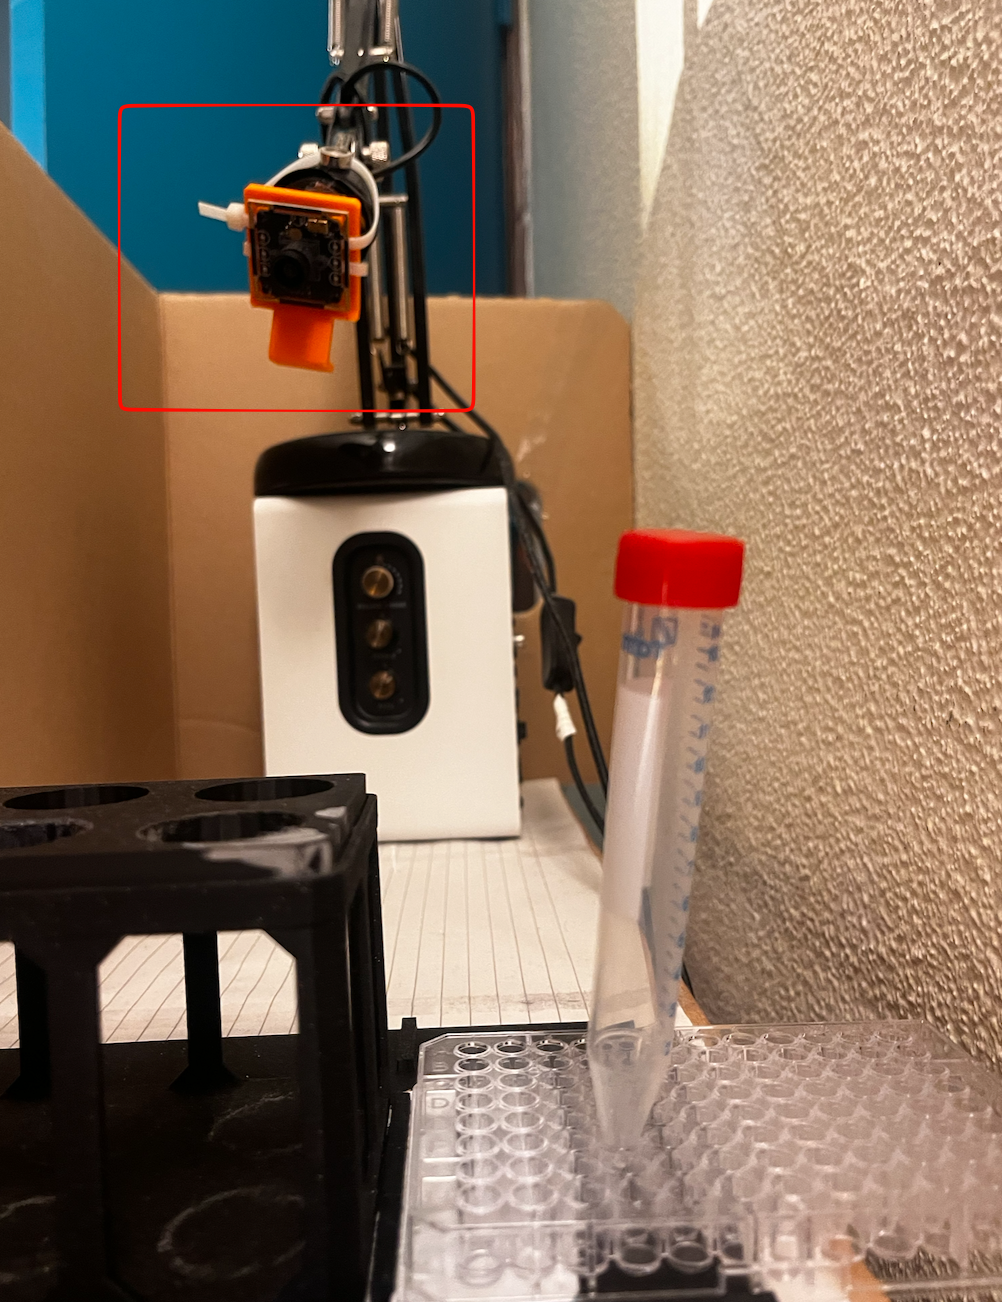
\includegraphics[width=0.5\textwidth]{images/camera_position.png}
    \caption{Overhead camera after a small deliberate displacement. Even this minor viewpoint shift caused the VLA to fail entirely.}
    \label{fig:camerapos}
\end{figure}

This was the biggest surprise. The model has basically no ability to handle camera angle changes. The pixel patterns have to match the training data almost exactly. In a real lab with the OT-2, this could work if you bolt the camera down before training and never touch it again.

%% ----------------------------------------------------------------
\section{Discussion}
\label{sec:discussion}
%% ----------------------------------------------------------------

\subsection{The Vision-Action Trade-off in Multi-task Learning}
\label{sec:visionaction}

The reason the model fails at new positions is something called the Vision-Action trade-off. When you train a VLA, one part (the vision backbone) learns to recognize objects, and another part (the action head) learns what movements to make. These two parts compete for the model's limited capacity.

The drop from 9/10 to 5/10 when I moved the tube to unseen positions fits this problem. The model seems to have learned the tube and the familiar training locations together, instead of fully separating what the tube looks like from where it appeared in the camera image. That is a softer explanation than saying it only memorised pixels, but it still explains why new positions caused trouble.

Here's the trade-off: adding more tasks or positions makes the vision backbone stronger (it sees more variety, learns better features). But if you have too many tasks or positions, the action head gets confused or runs out of capacity to store them all.

\begin{table}[H]
\centering
\renewcommand{\arraystretch}{1.3}
\begin{tabular}{@{}p{0.22\textwidth}p{0.72\textwidth}@{}}
\toprule
\textbf{Component} & \textbf{What happens when you add more tasks or positions} \\ \midrule
Vision backbone     & Gets better. Sees more variety, learns to recognize objects, not just memorize pixels. \\
Action head         & Can get worse. If tasks are too similar, the model confuses them. If there are too many, it runs out of space. \\
Small models        & No fixed task limit was found in the literature. The safer claim is that task capacity depends on model size, pretraining, data balance, replay, and the fine-tuning method; the practical risk is interference between behaviours, not a proven numeric ceiling \parencite{liu2026forgetting, romer2026clare}. \\ \bottomrule
\end{tabular}
\caption{The Vision-Action trade-off: adding more variation can help visual generalisation while also making the action mapping harder.}
\label{tab:visionaction}
\end{table}

To fix this for my task, I could:

\textbf{Option 1: Prompted multi-position training.} Instead of one generic prompt for all demonstrations, I could record more episodes from clearly different regions of the grid and give them different task prompts, such as \texttt{"Pipe in hole from left slot"}, \texttt{"Pipe in hole from centre slot"}, or \texttt{"Pipe in hole from right slot"}. This uses the VLA's language conditioning as a switch while keeping the overall behaviour the same.

\textbf{Option 2: Data augmentation.} Crop images randomly, zoom in and out, change colors. This tricks the model into being robust to position shifts without needing to run the robot 100 more times.

Both approaches target the root cause: the visual side saw too narrow a set of positions. More positional variety, either real or synthetic, should help it respond to a wider part of the grid.

\subsection{Gripper Design Constraints}
\label{sec:gripper}

One consistent problem across all tests was the gripper design. The SO-101 has an angular or scissor gripper where the fingers pivot around a pin. For a cylindrical tube, this means it grabs with just a single line of contact instead of squeezing evenly around the tube.

\begin{table}[H]
\centering
\renewcommand{\arraystretch}{1.2}
\begin{tabular}{@{}p{0.18\textwidth}p{0.37\textwidth}p{0.37\textwidth}@{}}
\toprule
\textbf{Property} & \textbf{Angular (Scissor)} & \textbf{Parallel} \\ \midrule
Mechanism       & Fingers pivot around a pin       & Fingers translate linearly \\
Ideal object    & Irregular shapes, tight spaces   & Cylinders, rectangular blocks \\
Contact area    & Single line along object         & Full surface contact \\
Force distribution & Uneven; tube can slip or rotate & Even; secure, predictable grip \\
OT-2 relevance  & Problematic for tubes/vials      & Standard for lab consumables \\ \bottomrule
\end{tabular}
\caption{Angular vs.\ parallel gripper comparison for cylindrical objects.}
\label{tab:grippers}
\end{table}

This gripper design is a problem because the tube slips or rotates when grabbed.\footnote{Examples: \url{https://youtube.com/shorts/hJA40Uhh7Cs}.} It's hard to know if the model is bad or just if the gripper can't hold the tube. Switching to a parallel gripper (where fingers close from opposite sides) would be the single biggest hardware improvement. That's the standard for lab automation anyway.

\subsection{What I Learned for Real Deployment}

Three things that matter if you want to actually use this in a lab:

\begin{enumerate}
    \item \textbf{Bolt the camera down.} Even small camera movements destroy performance. Friction clamps don't work.
    \item \textbf{Collect more prompted demonstrations.} Use imitation-learning data from different regions of the grid, and assign prompts that describe those regions, so the VLA has a better chance of handling larger position changes.
    \item \textbf{Use a parallel gripper.} The scissor gripper slips too much. The model can't fix that.
\end{enumerate}

%% ----------------------------------------------------------------
\section{Limitations and Future Work}
\label{sec:limitations}
%% ----------------------------------------------------------------

\subsection{Current Limitations}

\textbf{Dataset size and coverage.} This is the core limitation. Fifty final episodes were enough to get a working baseline, but not enough to make the model reliable across larger position changes. When the tube was in an unseen slot, the model still often moved toward familiar training regions.

To fix this, I would collect 150-200 better planned episodes from a wider range of grid positions, and I would use prompts that encode the starting region or context. The goal is not to record every possible slot forever, but to give the model enough imitation examples from meaningfully different locations that the prompt can help separate them. Alternatively, use data augmentation, such as random crops, zoom, and color shifts, to synthetically create position variation without running the robot more times.

\textbf{Viewpoint rigidity.} The camera-displacement test (Section~\ref{sec:camerapos}) showed that moving the overhead camera just a few centimetres completely breaks the model. This means every training run is brittle: if the camera shifts even slightly after data collection, performance can collapse. Mitigations: (1) multi-view training with 3 rigidly mounted cameras at different angles, (2) synthetic augmentation of camera viewpoints during training to build viewpoint-invariant features.

\textbf{Angular gripper.} The scissor gripper's single-line contact causes slippage and rotation (Section~\ref{sec:gripper}). This is a measurement problem: when the model fails, I can't tell if it's because the policy is bad or the gripper dropped the tube. A parallel gripper would give a cleaner signal about actual policy performance and is industry-standard for lab automation. This would also likely improve success rates, since the tube wouldn't slip.

\subsection{Bigger Models}

SmolVLA was the right choice for this project because inference had to run on my MacBook. But for a real lab with GPUs, a larger NVIDIA GR00T model would be worth testing \parencite{nvidia2026groot}. The trade-off is that inference would need to run on a GPU workstation, Jetson, or cluster-connected setup, not only on the MacBook. The good news is that both model families use robot demonstration data in a similar format, so the final 50 episodes could still be useful as a starting point.

\subsection{Roadmap to Deployment}

My results show VLAs can work on this task, but only under very specific conditions. Here's what you'd need to fix the key problems I found:

\begin{itemize}
    \item \textbf{Multiple rigidly mounted cameras (3 angles):} This directly addresses the viewpoint rigidity problem (Section~\ref{sec:camerapos}). Multi-angle training would make the model more robust to small camera shifts. It also gives the vision backbone richer 3D context.

    \item \textbf{Prompted position coverage (150-200 episodes):} Collect examples from clearly different grid regions and assign prompts that describe those regions. This should reduce the 9/10 to 5/10 drop without pretending that every possible slot has to be recorded exhaustively.

    \item \textbf{Parallel gripper:} Replaces the scissor gripper so the tube doesn't slip. Gives clean measurements of whether failures are policy-related or hardware-related. Industry standard for labs.

    \item \textbf{Controlled lighting:} A light booth or LED ring eliminates lighting as a variable. This was not a major problem here (Section~\ref{sec:lighting}), but it matters for consistency between training and deployment.

    \item \textbf{Multi-task curriculum (same task, different rack types):} Once you master "pipe in hole" with a standard rack, train on tubes in different container sizes and layouts. This keeps the action head focused on grasping while the vision backbone learns what a tube is across contexts.
\end{itemize}

With these changes, you'd have a real lab-deployment setup with robust perception, prompted data coverage, and hardware that doesn't introduce noise. That's when VLA-based robot control becomes genuinely useful for chemistry-lab automation.

\subsection{The Orchestrator Pattern: Beyond Single-Task VLAs}

One useful insight from recent work \parencite{ruiz2026toddler} is that VLAs are not general world models. They are fundamentally imitation-learning policies conditioned on task names. The practical setup is to combine a VLA with an orchestrator model that monitors the environment and decides which VLA action to invoke.

In that work, Gemini 3 Flash acted as the orchestrator: it tracked the game state, counted pieces, detected when wildcard die faces were rolled, and strategically commanded the VLA to execute the right motor primitives. The VLA (SmolVLA on an SO-101) did not need to understand game rules or strategy. It only needed to execute well-defined motor behaviors when told.

This pattern is especially useful for chemistry-lab automation:

\begin{itemize}
    \item \textbf{Finite action space:} A chemistry lab has a limited set of atomic operations (pipette, transfer tube, centrifuge, seal plate). A VLA can master each as a named task.
    \item \textbf{Finite failure modes:} Lab errors are predictable: dropped tubes, clogged tips, contamination. An orchestrator can detect these and decide whether to retry, skip, or alert the operator.
    \item \textbf{Protocol compliance:} The orchestrator (an LLM) understands the chemistry protocol, current deck state, and what comes next. The VLA is a motor executor, not a planner.
\end{itemize}

That matches what I saw in a simpler way: I should not expect the VLA to reason through a full lab protocol. A more realistic setup is to let another model choose the next named action, while the VLA only executes the low-level movement it was trained for. This keeps the motor policy smaller and makes failures easier to debug.

%% ----------------------------------------------------------------
\section{Conclusion}
\label{sec:conclusion}
%% ----------------------------------------------------------------

In this project I wanted to test a practical question for chemistry-lab automation: can a compact VLA handle the position and environment changes you would see in an OT-2-like setup? My results give a qualified yes.

Under training-matched conditions the model succeeded in 9 out of 10 trials, which suggests that tube manipulation with a compact VLA is possible on consumer hardware. The drop to 5 out of 10 with unseen positions shows the limitation: the policy stayed too tied to the positions it saw during training. The camera-displacement test failed completely, showing that viewpoint control is just as important as the model itself. These are not necessarily fundamental flaws, but they are serious engineering problems.

Three actionable takeaways emerge:
\begin{enumerate}
    \item \textbf{Fix cameras rigidly before data collection.} Even small shifts destroy performance.
    \item \textbf{Collect broader prompted demonstrations.} More imitation data from different grid regions should be paired with prompts that mark those regions.
    \item \textbf{Use a parallel gripper.} The scissor gripper introduces noise orthogonal to the policy.
\end{enumerate}

VLA-based robot control for chemistry labs is not yet a drop-in replacement for hard-coded OT-2 scripts. But the gap between proof-of-concept and deployment is closing. With the infrastructure improvements outlined in Section~\ref{sec:limitations}, and with the task-naming framework (upstream LLM normalisation) from Section~\ref{sec:background}, the first genuinely useful VLA deployment in a real chemistry lab is within reach.

\printbibliography

%% ----------------------------------------------------------------
\appendix
\section{Training Curves}
\label{app:training}
%% ----------------------------------------------------------------

This appendix reproduces the individual training metrics from the Weights \& Biases dashboard, summarised in Section~\ref{sec:smolvla}. The final training run was launched on a compute node with four NVIDIA A100 40\,GB GPUs, with the process using one GPU.

\begin{figure}[H]
    \centering
    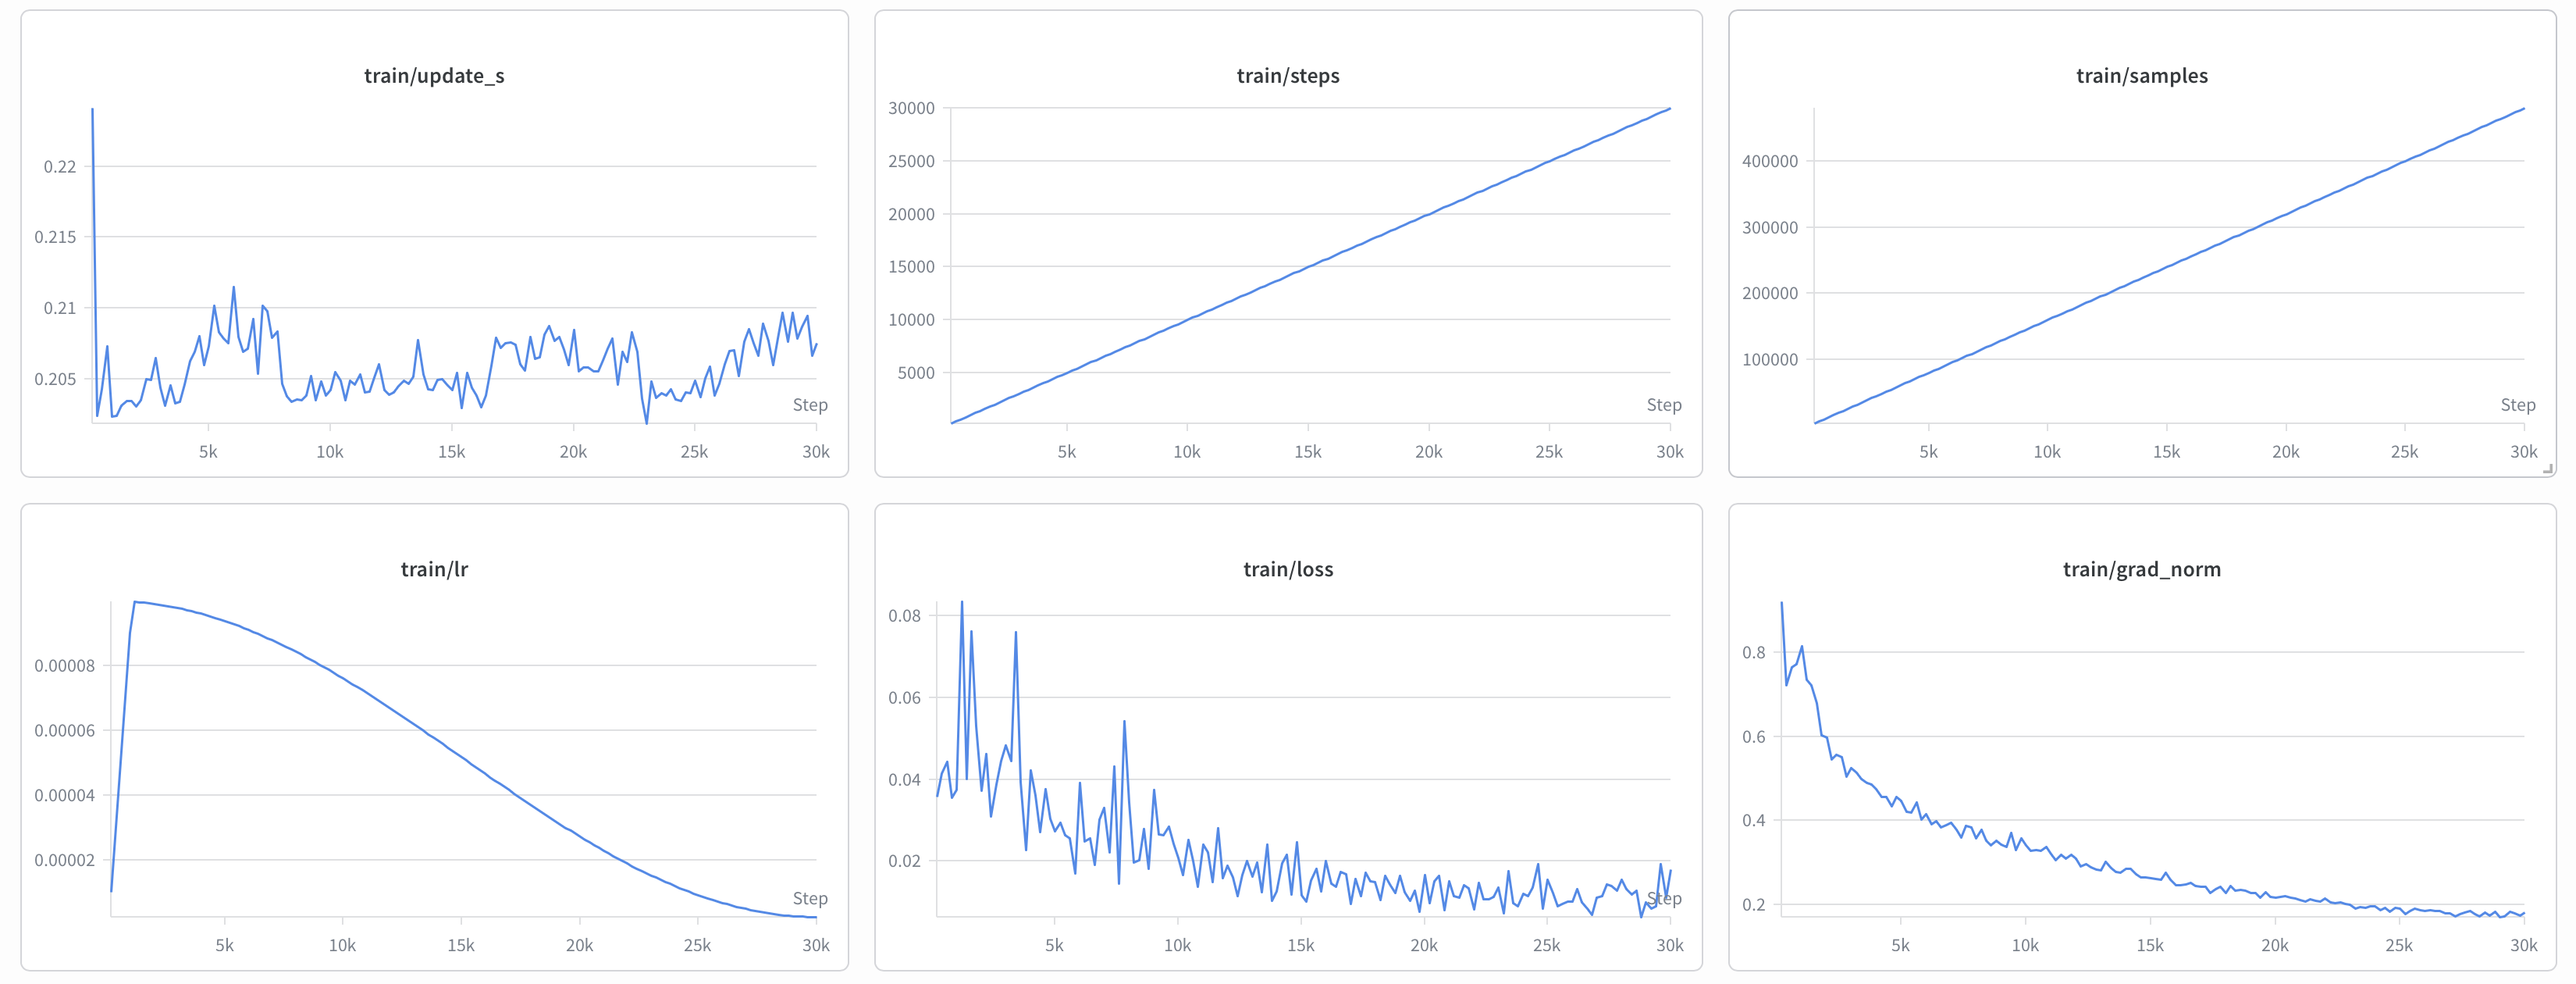
\includegraphics[width=\textwidth]{images/training_loss_1.png}
    \caption{Training dashboard overview showing update time, steps, samples, learning rate, training loss, and gradient norm.}
    \label{fig:training-overview}
\end{figure}

\begin{figure}[H]
    \centering
    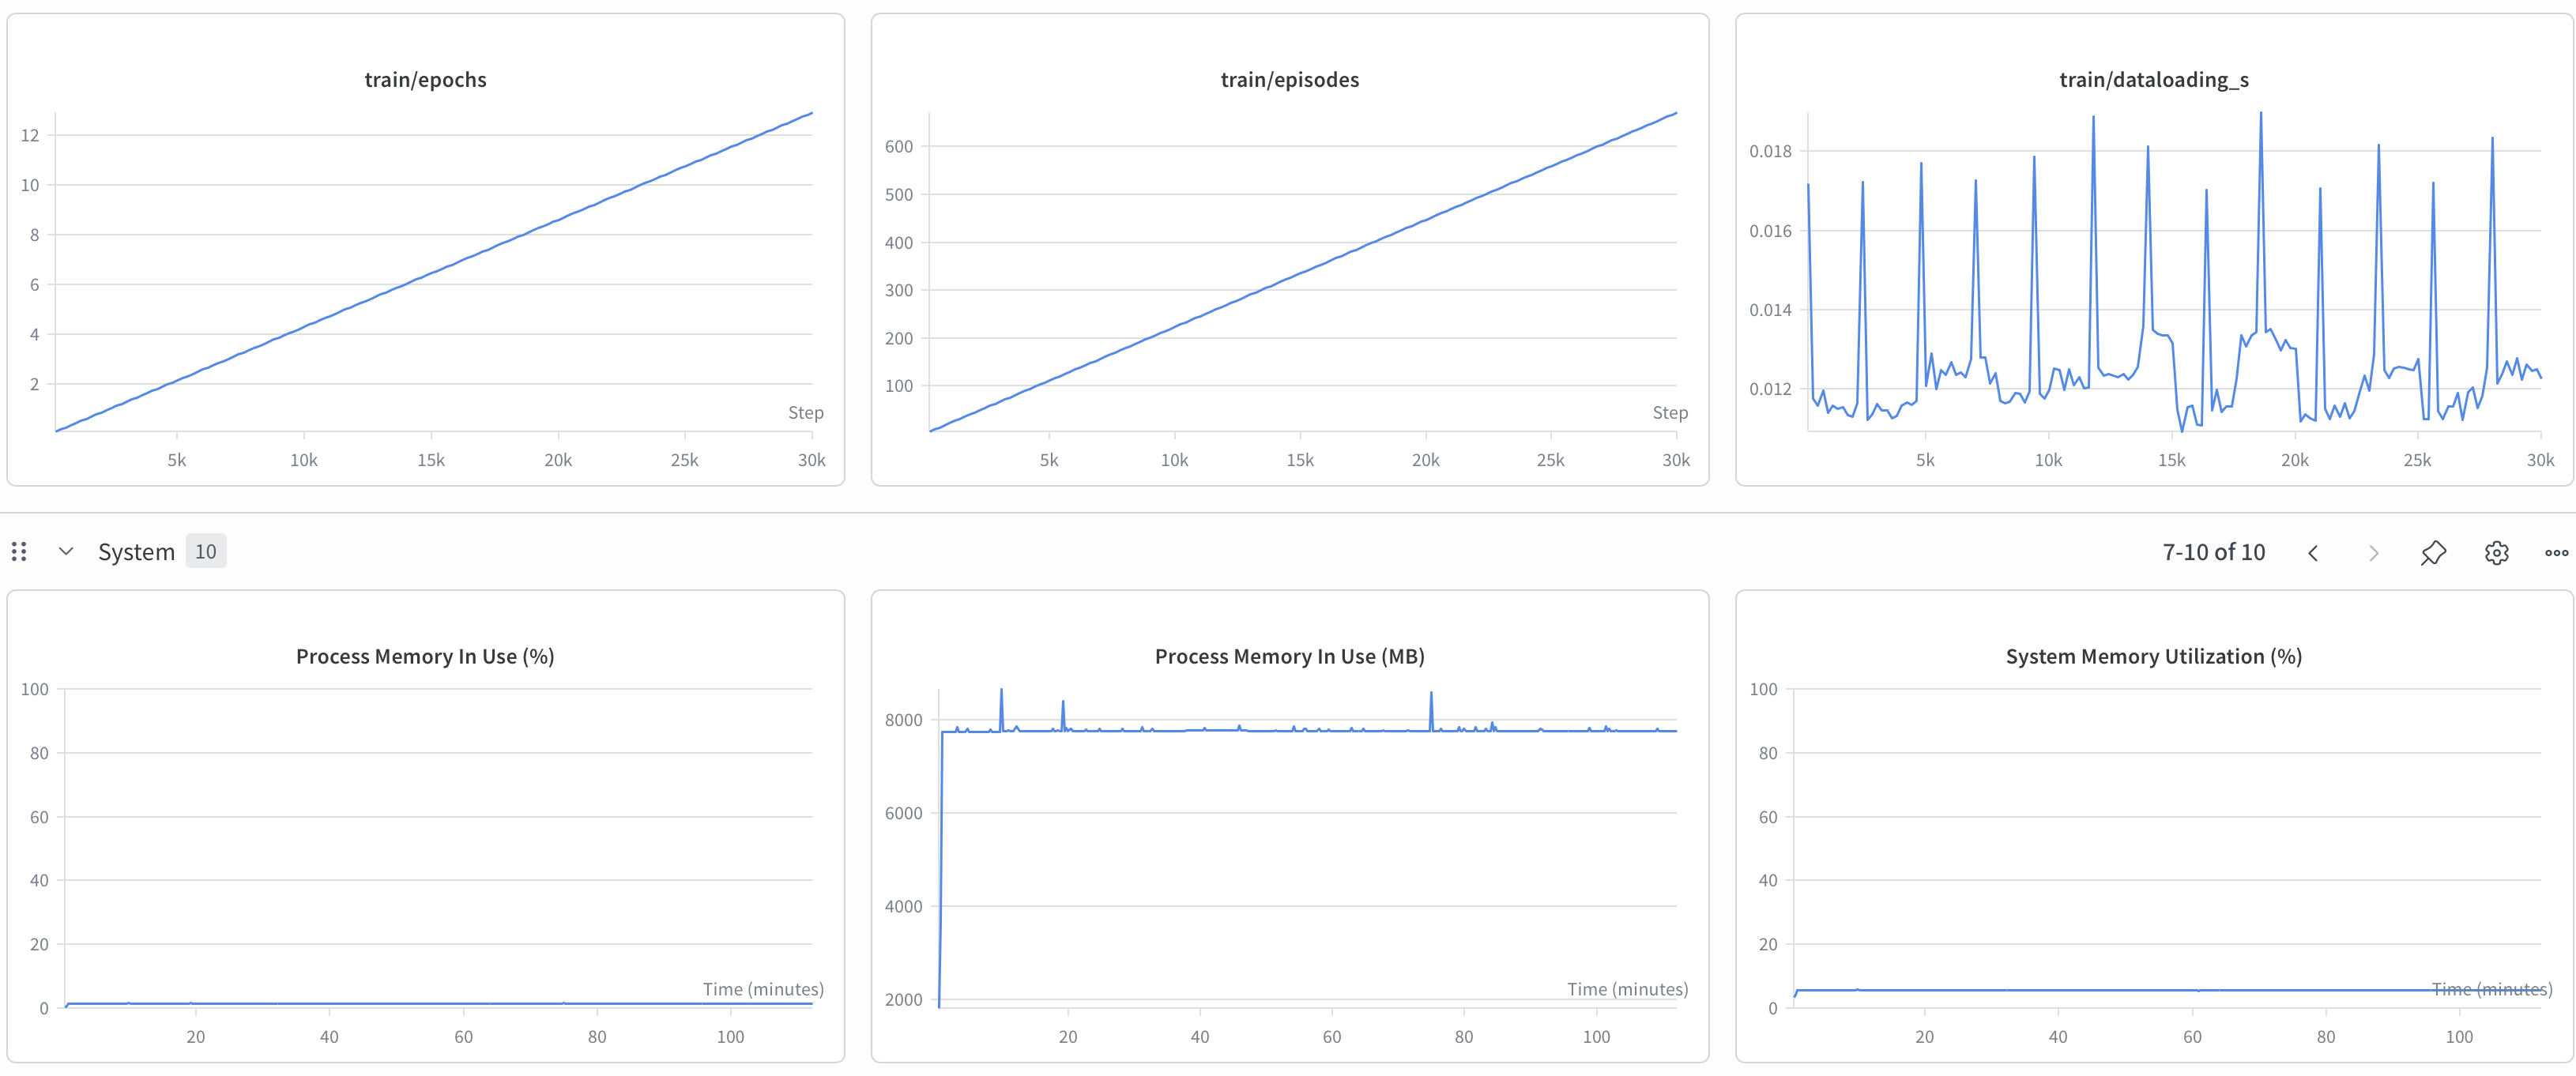
\includegraphics[width=\textwidth]{images/training_loss_2.png}
    \caption{Epoch, episode, data-loading, and system-memory metrics during training.}
    \label{fig:system-overview}
\end{figure}

\begin{figure}[H]
    \centering
    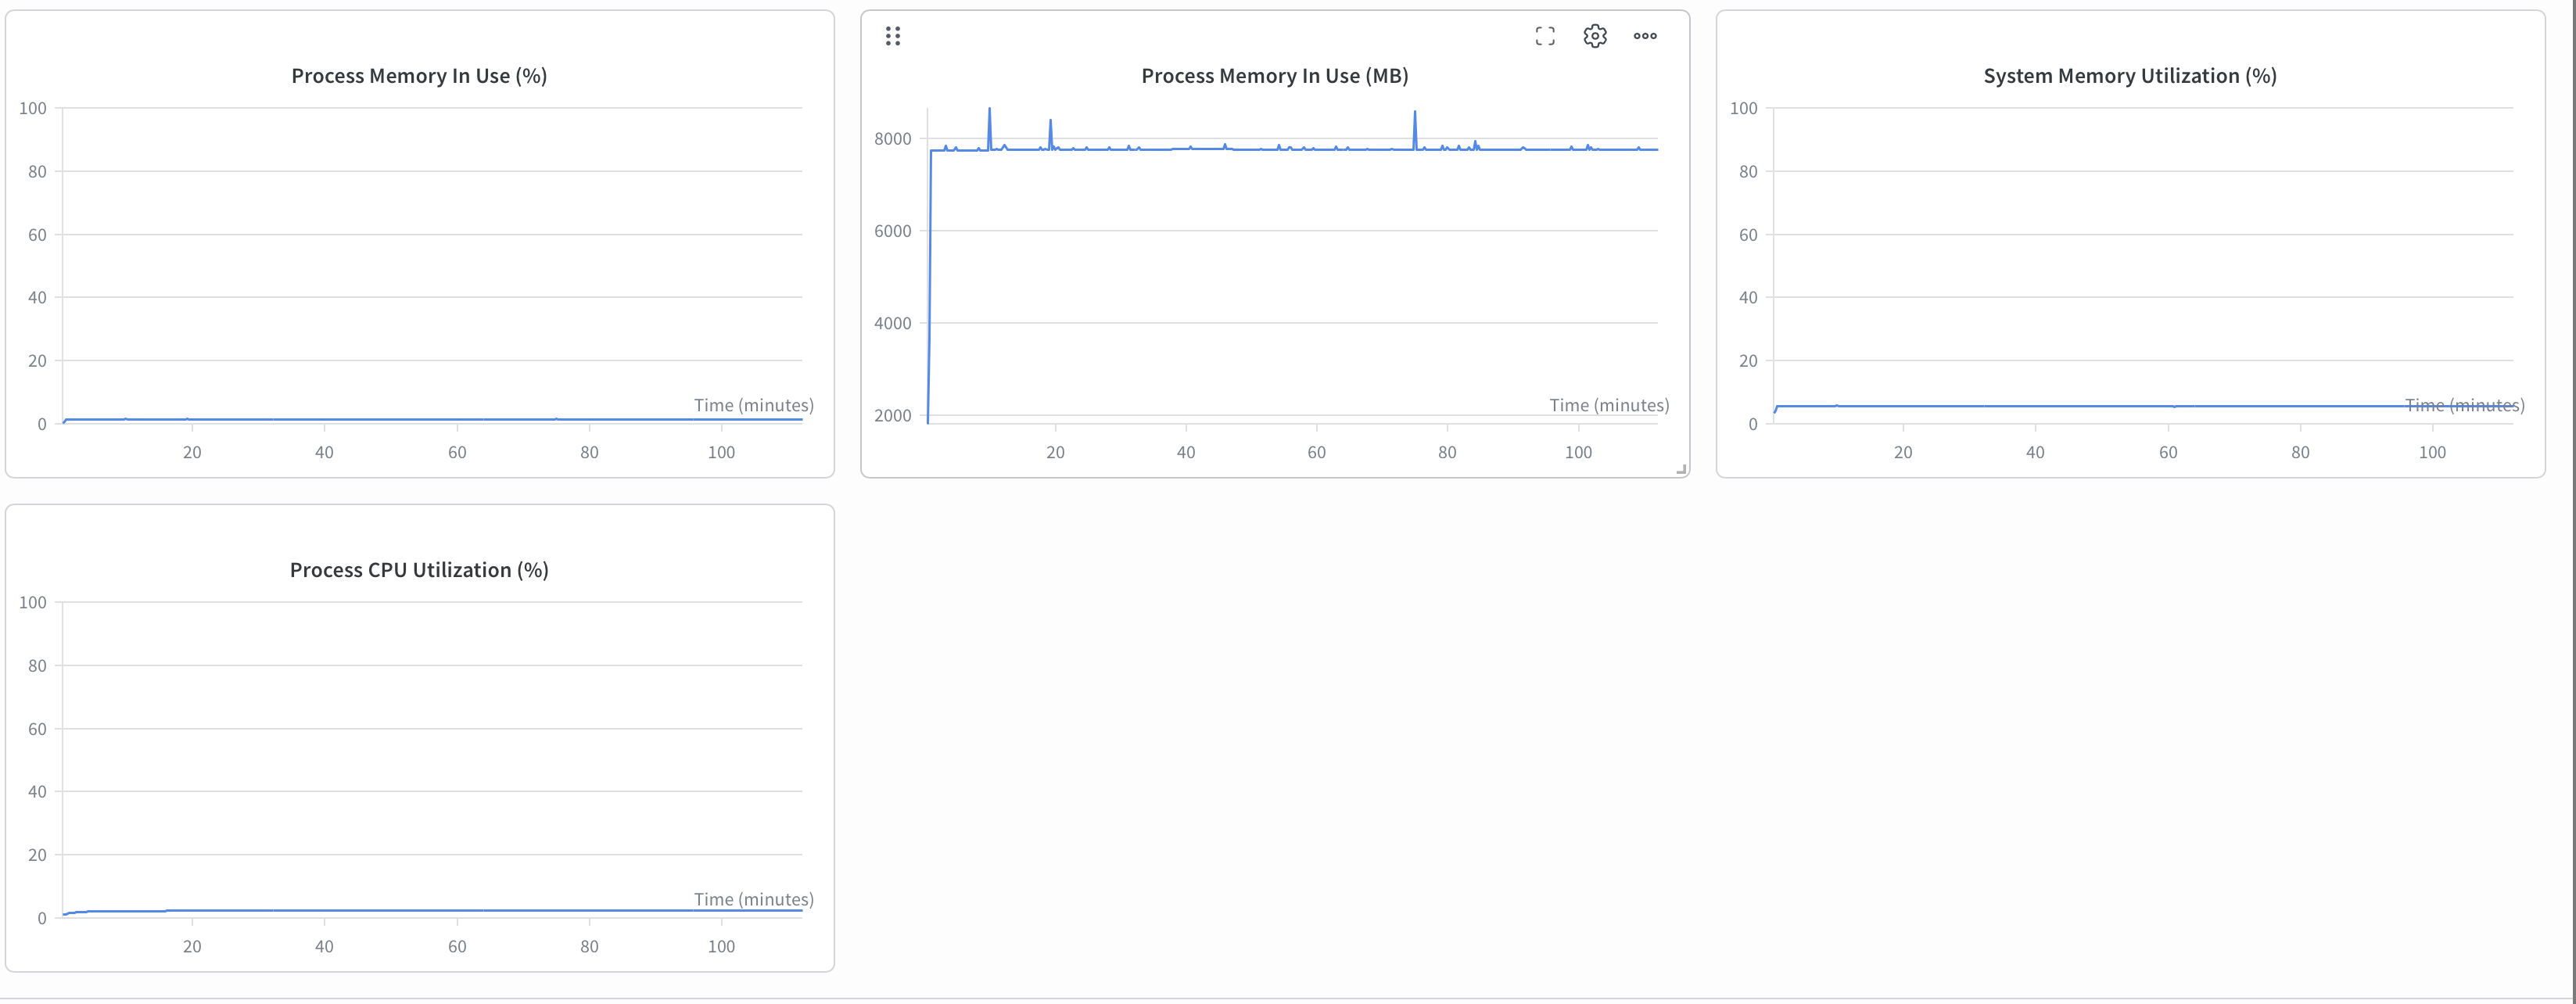
\includegraphics[width=\textwidth]{images/training_loss_3.png}
    \caption{Process memory and CPU utilisation during training.}
    \label{fig:process-resources}
\end{figure}

\begin{figure}[H]
    \centering
    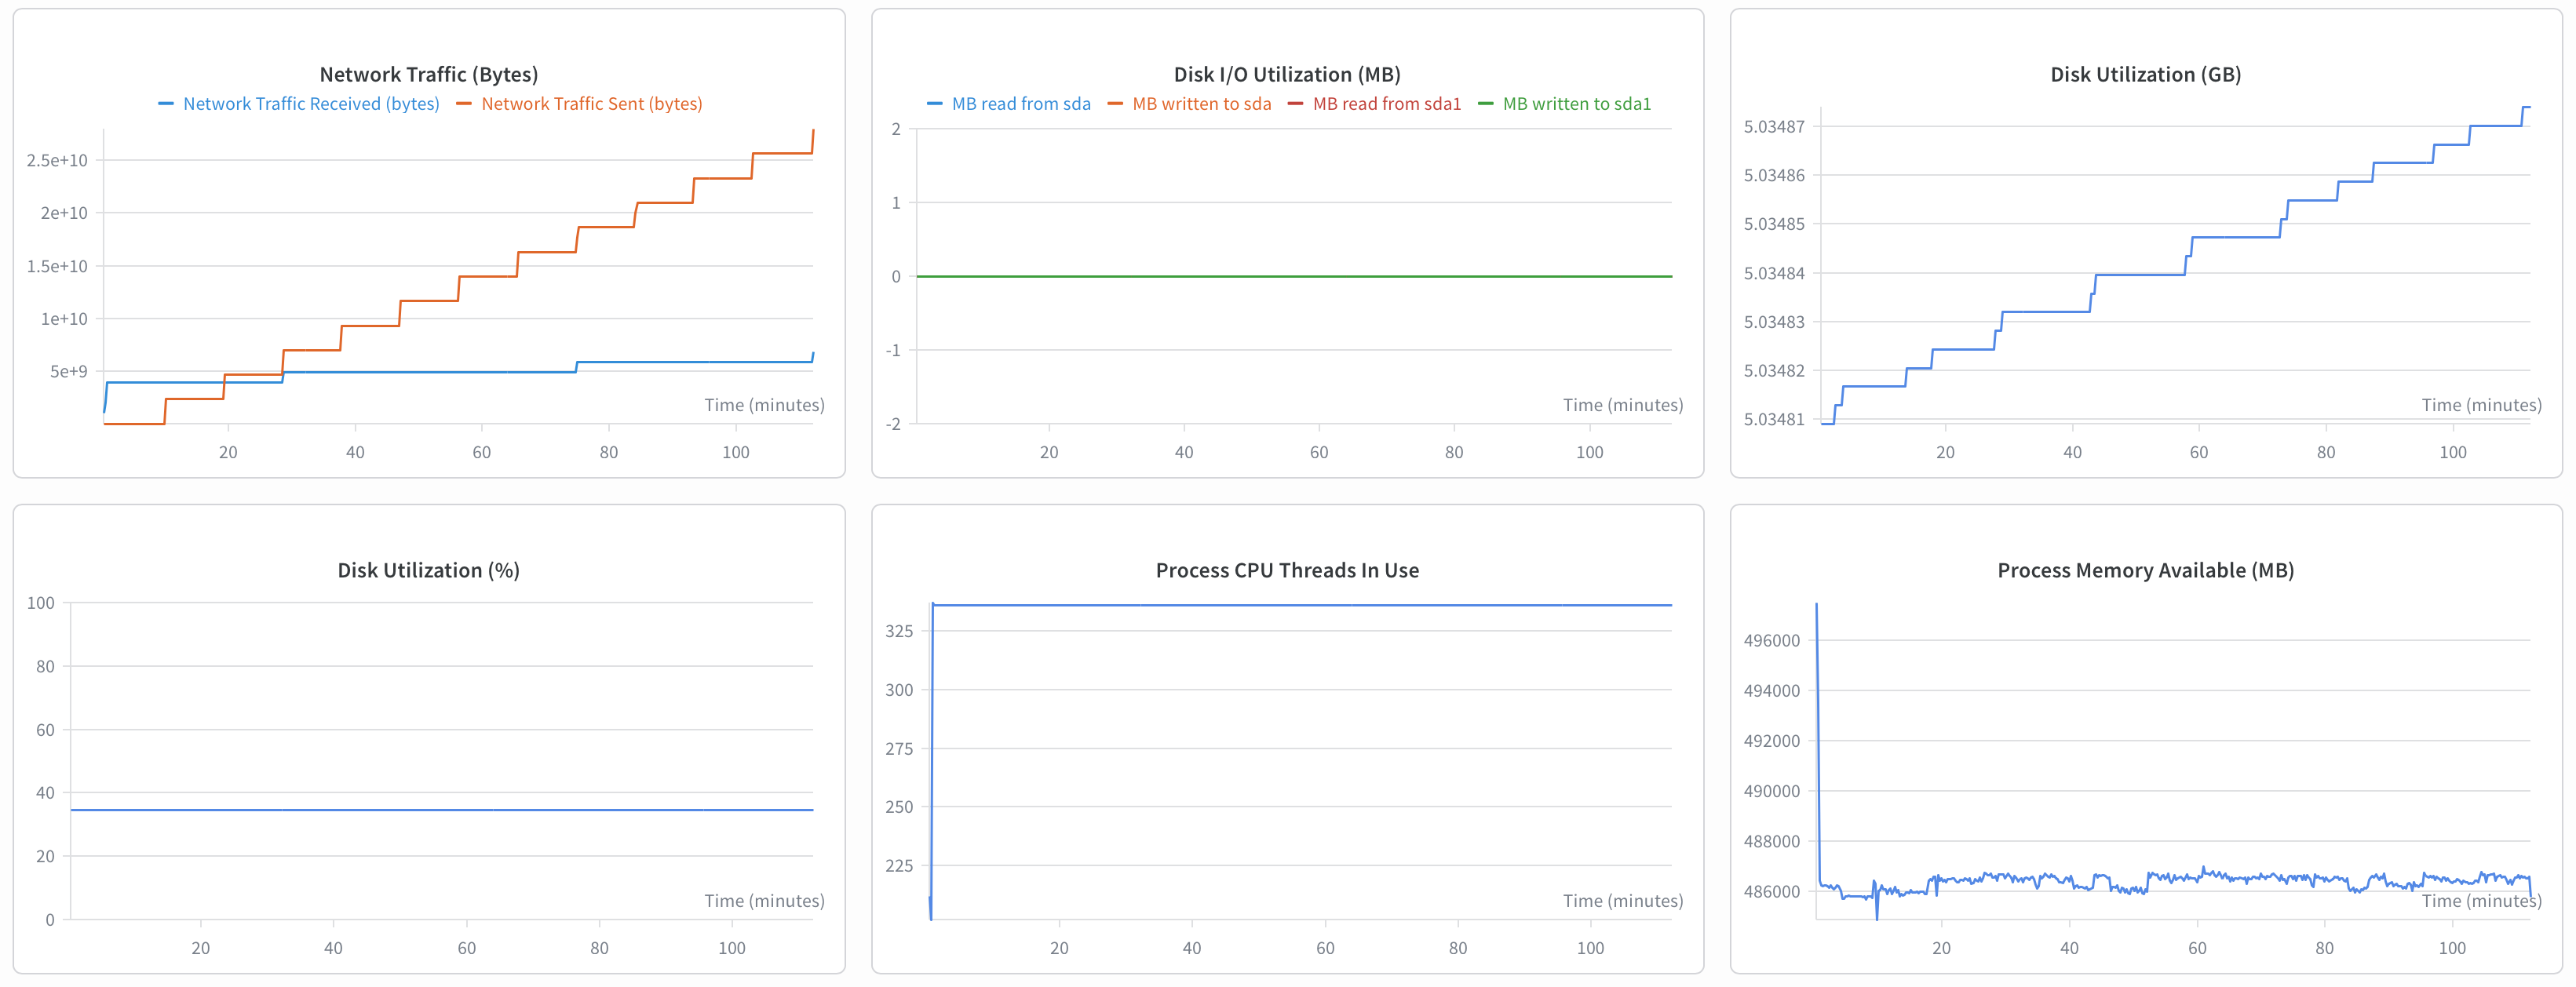
\includegraphics[width=\textwidth]{images/training_loss_4.png}
    \caption{Network, disk, thread, and memory-availability counters from the training node.}
    \label{fig:node-io}
\end{figure}

\end{document}
